\documentclass[11pt]{article} 
\usepackage{amsmath}
\usepackage{amsfonts}
\usepackage{amssymb}
\usepackage{geometry}
\geometry{a4paper, margin=1in}
\usepackage{graphicx}
\usepackage[hidelinks]{hyperref}
\usepackage{amsthm}
\usepackage{tikz}
\usepackage{subcaption}
\usetikzlibrary{positioning}
\usepackage{pgfplots} 
\usepackage[ruled,vlined]{algorithm2e} 
\usepackage{dsfont}
\usepackage{graphicx}
\usepackage{mathdesign}
\usepackage{float}
\usepackage{todonotes} 
\usepackage{empheq}
\usepackage{array}
\usepackage[ruled,vlined]{algorithm2e} 
\usepackage[many]{tcolorbox}    	% for COLORED BOXES (tikz and xcolor included)



\newtcolorbox{boxA}{
    fontupper = \bf,
    boxrule = 1.5pt,
    colframe = black % frame color
}


\setlength{\parindent}{0pt}
\numberwithin{equation}{section}


\newcommand\mycommfont[1]{\footnotesize\ttfamily\textcolor{blue}{#1}}
\newcommand\defeq{\stackrel{\mathclap{\normalfont\mbox{def}}}{=}}
\SetCommentSty{mycommfont}

\DeclareMathOperator*{\argmax}{argmax}
\DeclareMathOperator*{\argmin}{argmin}



\newtheoremstyle{boldStyle}%                % Name
  {}%                                     % Space above
  {}%                                     % Space below
  {\itshape}%                                     % Body font
  {}%                                     % Indent amount
  {\bfseries}%                            % Theorem head font
  {}%                                    % Punctuation after theorem head
  {\newline}                              % Space after theorem head, new line
  {\thmname{#1}\thmnumber{ #2}\thmnote{ (#3)}}%                                     % Theorem head spec (can be left empty, meaning `normal')


\theoremstyle{boldStyle}
\newtheorem{theorem}{Theorem}[section]
\newtheorem{lemma}{Lemma}[section]
\newtheorem{definition}{Definition}[section]
\newtheorem{corollary}{Corollary}[section]
\newtheorem{claim}{claim}[section]
\newtheorem{example}{Example}[section]


\newtheorem*{claim*}{Claim}
\newtheorem*{lemma*}{Lemma}
\newtheorem*{corollary*}{Corollary}
\newtheorem*{remark*}{Remark}
\newtheorem*{example*}{Example}
\newtheorem*{examples*}{Examples}
\newtheorem*{definition*}{Definition}



\title{
    \huge Behaviour of Sequential Predictors of Binary Sequences\\
    \vspace{10pt}
}

\author{T. M. Cover}

\date{Publishing House of the Czechoslovak Academy of Sciences, Prague 1967}



\begin{document}
\maketitle

% * * * * * * * * * * * * * * * * * * * * * * * * 
% * * * * * * * * * * * * * * * * * * * * * * * * 
% * * * * * * * * * * * * * * * * * * * * * * * * 
% * * * * * * * * * * * * * * * * * * * * * * * * 
% * * * * * * * * * * * * * * * * * * * * * * * * 
% * * * * * * * * * * * * * * * * * * * * * * * * 
% * * * * * * * * * * * * * * * * * * * * * * * * 
% * * * * * * * * * * * * * * * * * * * * * * * * 
% * * * * * * * * * * * * * * * * * * * * * * * * 
% * * * * * * * * * * * * * * * * * * * * * * * * 
% * * * * * * * * * * * * * * * * * * * * * * * * 
% * * * * * * * * * * * * * * * * * * * * * * * * 
% * * * * * * * * * * * * * * * * * * * * * * * * 
% * * * * * * * * * * * * * * * * * * * * * * * * 
% * * * * * * * * * * * * * * * * * * * * * * * * 
% * * * * * * * * * * * * * * * * * * * * * * * * 
% * * * * * * * * * * * * * * * * * * * * * * * * 
% * * * * * * * * * * * * * * * * * * * * * * * * 
% * * * * * * * * * * * * * * * * * * * * * * * * 
\section{Introduction}

This paper explores the effectiveness of sequential predictors on finite binary sequences. 
Prior work by Robbins, Hannan, and Blackwell has demonstrated algorithms capable of asymptotically achieving high scores by leveraging 
the empirical distribution of the sequences. Fogel has notably extended this by adapting the predictive model based on the sequence observed, 
achieving near-perfect accuracy on sequences displaying non-random patterns, such as prime numbers. This study investigates the capacity of sequential 
predictors to consistently generate high scores across a broad spectrum of sequences, delving into the inherent limits and potential of 
such algorithms in systematic and non-random environments.


% * * * * * * * * * * * * * * * * * * * * * * * * 
% * * * * * * * * * * * * * * * * * * * * * * * * 
% * * * * * * * * * * * * * * * * * * * * * * * * 
% * * * * * * * * * * * * * * * * * * * * * * * * 
% * * * * * * * * * * * * * * * * * * * * * * * * 
% * * * * * * * * * * * * * * * * * * * * * * * * 
% * * * * * * * * * * * * * * * * * * * * * * * * 
% * * * * * * * * * * * * * * * * * * * * * * * * 
% * * * * * * * * * * * * * * * * * * * * * * * * 
% * * * * * * * * * * * * * * * * * * * * * * * * 
% * * * * * * * * * * * * * * * * * * * * * * * * 
% * * * * * * * * * * * * * * * * * * * * * * * * 
% * * * * * * * * * * * * * * * * * * * * * * * * 
% * * * * * * * * * * * * * * * * * * * * * * * * 
% * * * * * * * * * * * * * * * * * * * * * * * * 
% * * * * * * * * * * * * * * * * * * * * * * * * 
% * * * * * * * * * * * * * * * * * * * * * * * * 
% * * * * * * * * * * * * * * * * * * * * * * * * 
% * * * * * * * * * * * * * * * * * * * * * * * * 
\section{Deterministic Predictors}

Consider the set of $2^n$ sequences $\Theta = (\Theta_1, \Theta_2, \ldots, \Theta_{n}) \in \{0, 1\}^n$.

At stage $k$, after the observation $\Theta_1, \Theta_2, \ldots, \Theta_{k-1}$, the prediction 1 or 0 will be made with probability $p_k$ and $1-p_k$ respectively.

A \textbf{sequential predictor} on $\{0, 1\}^n$ will be completely specified by the set of functions 
\[
    p_1, p_2(\Theta_1), p_3(\Theta_1, \Theta_2), \ldots, p_n(\Theta_1, \Theta_2, \ldots, \Theta_{n-1})
\]
taking values in $[0, 1]$.
\begin{itemize}
    \item If the $p_i$s are restricted to $\{0, 1\}$, the predictor is called a \textbf{deterministic predictor}.
    \item If the $p_i$s are independent of the $\Theta$s, the predictor is called a \textbf{memoryless predictor}.
    \item If the $p_i$s are also independent of $i$, the predictor is called a \textbf{constant/time invariant predictor}.
\end{itemize}

Let $\delta = (\delta_1, \delta_2, \ldots, \delta_n) \in \{0, 1\}^n$ be the sequence of R.V.s resulting from the predictor $p = (p_1, p_2, \ldots, p_n)$ and the sequence $\Theta \in \{0, 1\}^n$.

Then the empirical average score (the fraction of correct predictions) is given by

\begin{align}
    s = \frac{1}{n} \sum_{i=1}^{n} ( \delta_i \Theta_i + (1 - \delta_i)(1 - \Theta_i) )
\end{align}

and the expected empirical average score is given by

\begin{align}
    \bar{s} = \mathbb{E}_{p}(s) =  \frac{1}{n} \sum_{i=1}^{n} \left( p_i \Theta_i + (1 - p_i)(1 - \Theta_i) \right) 
\end{align}

\begin{boxA}
    \textbf{(I)} Any sequential deterministic predicator attains a score of $\frac{k}{n}$ on precisely $\binom{n}{k}$ sequences in $\{0, 1\}^n$ where $k \in [n]$.
    For any deterministic predictor, there exists a sequence upon which a score of 0 is attained.
\end{boxA}


% * * * * * * * * * * * * * * * * * * * * * * * * 
% * * * * * * * * * * * * * * * * * * * * * * * * 
% * * * * * * * * * * * * * * * * * * * * * * * * 
% * * * * * * * * * * * * * * * * * * * * * * * * 
% * * * * * * * * * * * * * * * * * * * * * * * * 
% * * * * * * * * * * * * * * * * * * * * * * * * 
% * * * * * * * * * * * * * * * * * * * * * * * * 
% * * * * * * * * * * * * * * * * * * * * * * * * 
% * * * * * * * * * * * * * * * * * * * * * * * * 
% * * * * * * * * * * * * * * * * * * * * * * * * 
% * * * * * * * * * * * * * * * * * * * * * * * * 
% * * * * * * * * * * * * * * * * * * * * * * * * 
% * * * * * * * * * * * * * * * * * * * * * * * * 
% * * * * * * * * * * * * * * * * * * * * * * * * 
% * * * * * * * * * * * * * * * * * * * * * * * * 
% * * * * * * * * * * * * * * * * * * * * * * * * 
% * * * * * * * * * * * * * * * * * * * * * * * * 
% * * * * * * * * * * * * * * * * * * * * * * * * 
% * * * * * * * * * * * * * * * * * * * * * * * * 
\section{Sequential Betting Systems}

% * * * * * * * * * * * * * * * * * * * * * * * * 
% * * * * * * * * * * * * * * * * * * * * * * * * 
% * * * * * * * * * * * * * * * * * * * * * * * * 
% * * * * * * * * * * * * * * * * * * * * * * * * 
% * * * * * * * * * * * * * * * * * * * * * * * * 
\subsection{Achievable Winnings in Sequential Betting}

A series of \(n\) bets \(b = (b_1, b_2, \ldots, b_n)\) is made by a gambler on the outcomes of a sequence \(\Theta = (\Theta_1, \Theta_2, \ldots, \Theta_n) \in \{0, 1\}^n\).
The gambler's net gain at bet \(k\) is \(b_k\) if \(\Theta_k = 1\) and \(-b_k\) if \(\Theta_k = 0\). Hence, his net winnings \(w(\Theta)\) using strategy \(b\) against sequence \(\Theta\) is
\begin{align} \label{eq:3.1}
    w(\Theta) = \sum_{k=1}^n \left(b_k \Theta_k - b_k(1 - \Theta_k)\right) = \sum_{k=1}^n b_k(2\Theta_k - 1),
\end{align}

where, in general, \(b_k\) will be a real valued function of \(\Theta\).

\medbreak

Notice that a gambler may win any preassigned amount \(w(\Theta)\) if \(\Theta\) is known a priori. For example, any \(w\) could be achieved with the betting system
\begin{equation} \label{eq:3.2}
    \begin{aligned}
        b_1 &= w(\Theta) \Theta_1 - w(\Theta)(1 - \Theta_1), \\
        b_2 &= b_3 = \ldots = b_n = 0.
    \end{aligned}
\end{equation}

However, if he knows only \(\Theta_1, \Theta_2, \ldots, \Theta_{k-1}\) when he must place his bet \(b_k\), his set of achievable winnings \(w\) on \(\{0, 1\}^n\) is limited. For, if \(\{b_1, b_2, \ldots, b_n\}\) achieves \(w\), then manipulation of the above sum, noting the functional independence of \(b_k\) and \(\Theta_k\), yields
\begin{align} \label{eq:3.3}
    w(\Theta_1, \ldots, \Theta_{n-1}, 1) + w(\Theta_1, \ldots, \Theta_{n-1}, 0) = 2 \sum_{k=1}^{n-1} b_k(2\Theta_k - 1),
\end{align}

and
\begin{align} \label{eq:3.4}
    w(\Theta_1, \ldots, \Theta_{n-1}, 1) - w(\Theta_1, \ldots, \Theta_{n-1}, 0) = 2b_n.
\end{align}

So, \(b_n\) is determined and \ref{eq:3.1} is replaced by \ref{eq:3.3} for the determination of \(b_{n-1}\). 

Proceeding, we find
\begin{align} \label{eq:3.5}
    \sum_{\Theta} w(\Theta) = 0
\end{align}

\textbf{Proof:}
\begin{align*}
    \sum_{\Theta} w(\Theta) &= \sum_{\Theta} \sum_{k=1}^n b_k(2\Theta_k - 1) \\
    &= \sum_{k=1}^n b_k \sum_{\Theta} (2\Theta_k - 1) \\
    &= \sum_{k=1}^n b_k \cdot 0 = 0.
\end{align*}

and 

\begin{align} \label{eq:3.6}
    b_k = (\frac{1}{2})^{n-k+1} \sum_{(\Theta_k, \Theta_{k+1}, \ldots, \Theta_n) \in \{0, 1\}^{n-k+1}} w(\Theta)(2\Theta_k - 1) \quad (k = 1, 2, \ldots, n).
\end{align}

\textbf{Proof:}

For \(k = n\), we need to show that
\begin{align*}
    b_n = \left(\frac{1}{2}\right) \sum_{\Theta_n \in \{0, 1\}} w(\Theta_1, \ldots, \Theta_{n-1}, \Theta_{n})(2\Theta_n - 1)
\end{align*}
we have from \ref{eq:3.4} that 
\begin{align*}
    &w(\Theta_1, \ldots, \Theta_{n-1}, 1) - w(\Theta_1, \ldots, \Theta_{n-1}, 0) = 2b_n, \\
    b_n &= \frac{1}{2}(w(\Theta_1, \ldots, \Theta_{n-1}, 1) - w(\Theta_1, \ldots, \Theta_{n-1}, 0)).
\end{align*}

\bigbreak

For general $b_k$ it holds that
\begin{align*}
    &\sum_{(\Theta_k, \ldots, \Theta_n)} w(\Theta_1, \ldots, \Theta_{k-1}, \Theta_{k}, \ldots, \Theta_n) (2\Theta_k - 1) = \\
    &\sum_{(\Theta_{k+1}, \ldots, \Theta_n)} w(\Theta_1, \ldots, \Theta_{k-1}, 1, \Theta_{k+1}, \ldots, \Theta_n) - w(\Theta_1, \ldots, \Theta_{k-1}, 0, \Theta_{k+1}, \ldots, \Theta_n)  = \\
    &2 \cdot b_k \cdot 2^{n-(k+1)+1} = 2 \cdot b_k \cdot 2^{n-k} = b_k \cdot 2^{n-k+1}
    \\ \Longrightarrow \\
    &b_k = \left(\frac{1}{2}\right)^{n-k+1} \sum_{(\Theta_k, \ldots, \Theta_n) \in \{0, 1\}^{n-k+1}} w(\Theta)(2\Theta_k - 1).
\end{align*}

\bigbreak

Hence, for $w(\Theta)$ to be achievable by a sequential betting scheme, it is necessary and sufficient (\ref{eq:3.5}) be satisfied.
The betting scheme achieving \(w\) is unique and is given by (\ref{eq:3.6}).

\begin{figure}[H]
    \centering
    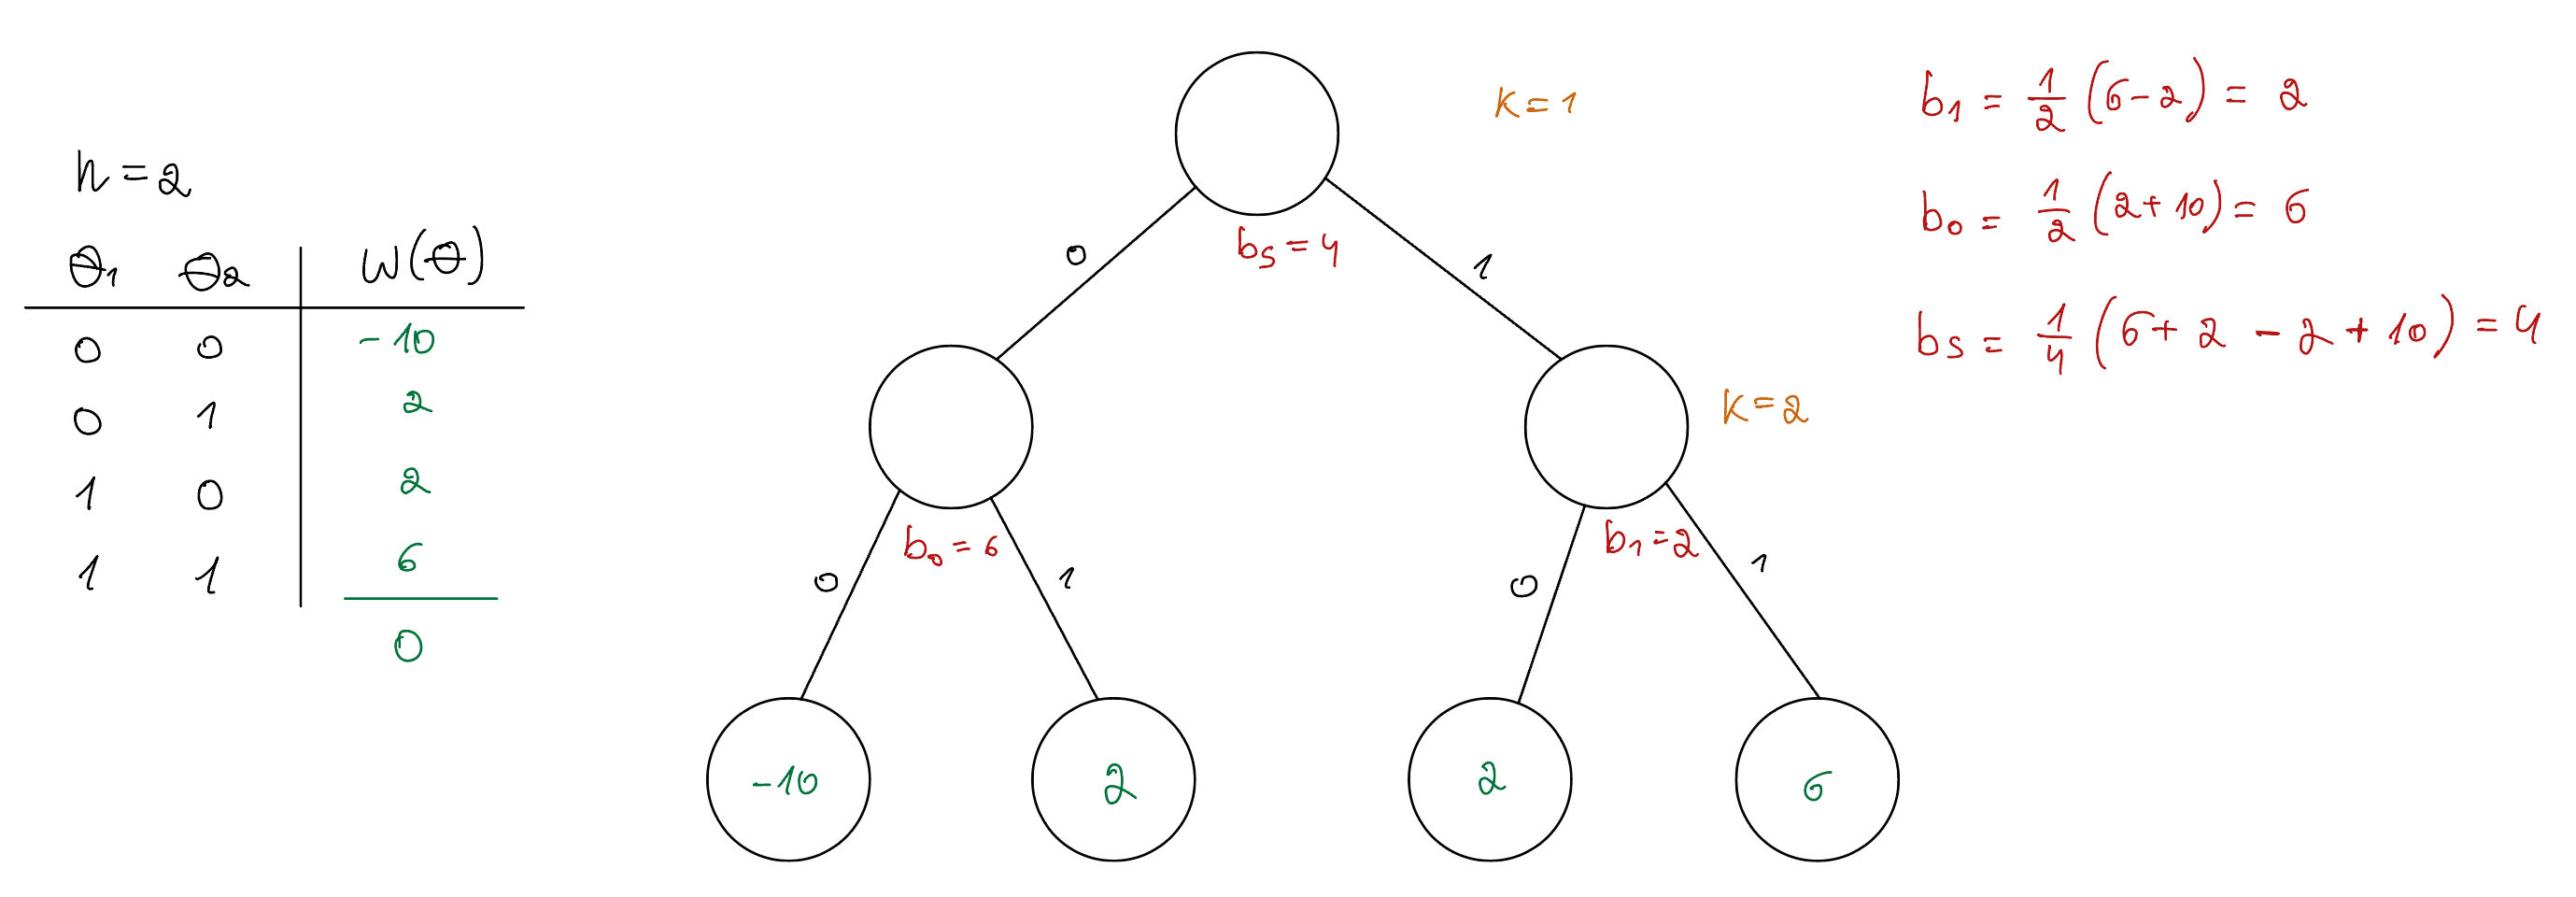
\includegraphics[width=\textwidth]{figs/achievable_winning.jpeg}
    \caption{Sequential Betting Scheme}
\end{figure}


\bigbreak

\textbf{Summary:}


Consider a betting strategy for a game against sequences: $\Theta = (\Theta_1, \Theta_2, \ldots, \Theta_n) \in \{0,1\}^n$, which allows the bet $b_k$ at stage $k$ to be some 
element in a subset $B_k$ of the collection $B$ of all functions from $\{0,1\}^n$ to $\mathbb{R}$. 
Let $w: \{0,1\}^n \rightarrow \mathbb{R}$ be a desired set of net winnings defined for each sequence $\Theta$ in $\{0,1\}^n$. 
As before, \ref{eq:3.1} expresses the net winnings $w(\Theta)$ as a function of $\{b_1, b_2, \ldots, b_n\}$. Then:

\begin{boxA}
    \textbf{(II)} Trivially, if $B_k = B$, any $w$ is achievable.
\end{boxA}

\begin{boxA}
    \textbf{(III)} If $B_k$ is the set of all functions in $B$ depending only on $\Theta_1, \Theta_2, \ldots, \Theta_{k-1}$, 
    then $w$ is achievable if and only if (\ref{eq:3.5}) is satisfied.
\end{boxA}

\begin{boxA}
    \textbf{(IV)} If, for $k = 1, 2, \ldots, n$, $B_k \subseteq B$ is the set of functions bounded in absolute value by $b$, depending only on $\Theta_1, \Theta_2, \ldots, \Theta_{k-1}$, 
    then $w$ is achievable if and only if
    \begin{align} \label{eq:3.7}
        \sum_{\Theta} w(\Theta) &= 0 
    \end{align}
    and if, for $k = 1, 2, \ldots, n$,
    \begin{align} \label{eq:3.8}
        \left|\left(\frac{1}{2}\right)^{n-k+1} \sum_{(\Theta_k, \Theta_{k+1}, \ldots, \Theta_n) \in \{0,1\}^{n-k+1}} w(\Theta)(2\Theta_k - 1)\right| &< b 
    \end{align}
    for every $(\Theta_1, \Theta_2, \ldots, \Theta_{k-1}) \in \{0, 1\}^{k-1}$. This is the sequential betting scheme with bounded bet size.
\end{boxA}




% * * * * * * * * * * * * * * * * * * * * * * * * 
% * * * * * * * * * * * * * * * * * * * * * * * * 
% * * * * * * * * * * * * * * * * * * * * * * * * 
% * * * * * * * * * * * * * * * * * * * * * * * * 
% * * * * * * * * * * * * * * * * * * * * * * * * 
\subsection{Winnings which are functions of $\sum_{i=1}^{n} \Theta_i$}


We may be interested in winnings $w$ which are functions only of $\sum_{i=1}^n \Theta_i$, the number of $1$'s in $\Theta$. In this case, define, for every $\Theta \in \{0, 1\}^n$,
\begin{equation} \label{eq:3.9}
    \hat{w} \left(\sum_{i=1}^n \Theta_i\right) = w(\Theta).
\end{equation}

Then the conditions of \ref{eq:3.7} and \ref{eq:3.8} become respectively
\begin{equation} \label{eq:3.10}
    \sum_{k=0}^n \binom{n}{k} \hat{w}(k) = 0
\end{equation}
and
\begin{equation} \label{eq:3.11}
    \left|b_k(i)\right| = \left|\left(\frac{1}{2}\right)^{n-k+1} \sum_{j=0}^{n-k} \left(\hat{w}(i+j+1) - \hat{w}(i+j)\right) \binom{n-k}{j}\right| < b
\end{equation}
For \(i = 0, 1, \ldots, k - 1\) and \(k = 1, 2, \ldots, n\) where
$b_k(i)$ is the bet at stage \(k\) when the sum of the first \(k - 1\) outcomes is \(i\).

\textbf{Proof:}

We start by expanding the expression from Equation \eqref{eq:3.8} under the assumption that $\hat{w} \left(\sum_{i=1}^n \Theta_i\right) = w(\Theta)$ from Equation \eqref{eq:3.9}:

\begin{align*}
    &\text{LHS of \eqref{eq:3.8}} = \left| b_k(i) \right| \\ 
    &= \left|\left(\frac{1}{2}\right)^{n-k+1} \sum_{(\Theta_k, \Theta_{k+1}, \ldots, \Theta_n) \in \{0,1\}^{n-k+1}} w(\Theta)(2\Theta_k - 1)\right| \\
    &= \left|\left(\frac{1}{2}\right)^{n-k+1} \sum_{j=0}^{n-k+1} \left(\sum_{(\Theta_k, \ldots, \Theta_n) \in \{0,1\}^{n-k+1} : \sum \Theta_i = j} w(\Theta) (2\Theta_k - 1)\right) \right| \\
    &= \left|\left(\frac{1}{2}\right)^{n-k+1} \sum_{j=0}^{n-k} \left( \sum_{(\Theta_{k+1}, \ldots, \Theta_n)} w(\Theta_1, \ldots, \Theta_k, 1, \Theta_{k+1}, \ldots, \Theta_n) - w(\Theta_1, \ldots, \Theta_k, 0, \Theta_{k+1}, \ldots, \Theta_n) \right) \right| \\
    &= \left|\left(\frac{1}{2}\right)^{n-k+1} \sum_{j=0}^{n-k} \left(\hat{w}(i+j+1) - \hat{w}(i+j)\right) \binom{n-k}{j}\right|,
\end{align*}
where the binomial coefficient $\binom{n-k}{j}$ counts the number of ways in which $\sum \Theta_i = j$ can occur.

The term inside the summation represents the change in winnings $\hat{w}$ when the count of 1's increases by one, hence reflecting the derivative (or difference) $\hat{w}(i+j+1) - \hat{w}(i+j)$. The multiplication by $\binom{n-k}{j}$ adjusts for the number of sequences that result in a particular sum $j$ of 1's among the last $n-k$ flips.

Thus, we have shown that:
\begin{equation*}
    \text{LHS of \eqref{eq:3.8}} = \text{RHS of \eqref{eq:3.11}},
\end{equation*}

\bigbreak

Now we will find a sufficient bound on $\left| b_k(i) \right|$ such that the conditions of \ref{eq:3.11} are satisfied.

Letting \(k = n\) in (3.11) we have the condition:
\begin{equation} \label{eq:3.12}
    \left |b_n(i) \right| = \frac{1}{2} \left| \hat{w}(i + 1) - \hat{w}(i)\right| < b
\end{equation}
for \(i = 0, 1, \ldots, n - 1\).

All other conditions of (3.11) are consequences of (3.12), since, assuming (3.12) true,
\begin{equation} \label{eq:3.13}
    \begin{aligned}
        \left|b_k(i)\right| &= \left| \left(\frac{1}{2}\right)^{n-k+1} \sum_{j=0}^{n-k} \left(w(i + j + 1) - w(i + j)\right) \binom{n-k}{j} \right| \leq \\
        &\left(\frac{1}{2}\right)^{n-k+1} \sum_{j=0}^{n-k} \binom{n-k}{j} 2b = b.
    \end{aligned}
\end{equation}

\begin{boxA}
\textbf{(V)} A terminal score \(\hat{w}\) depending only on \(\sum_{i=1}^n \Theta_i\) is achievable by a sequential betting scheme with bounded bet size \(b\) if and only if
\begin{equation} \label{eq:3.14}
    \sum_{k=0}^n \binom{n}{k} \hat{w}(k) = 0
\end{equation}
and
\begin{equation} \label{eq:3.15}
    \left| \hat{w}(k + 1) - \hat{w}(k)\right| < 2b, \quad k = 1, 2, \ldots, n - 1.
\end{equation}
\end{boxA}



% * * * * * * * * * * * * * * * * * * * * * * * * 
% * * * * * * * * * * * * * * * * * * * * * * * * 
% * * * * * * * * * * * * * * * * * * * * * * * * 
% * * * * * * * * * * * * * * * * * * * * * * * * 
% * * * * * * * * * * * * * * * * * * * * * * * * 
\subsection{Examples}

\subsubsection{Example 1 - foreknowledge of a sequence which will not occur}

Consider a gambler betting on a binary sequence of length \(n\), consisting of 1's and 0's. 
The gambler can choose his bet amount at each stage, based on the sequence observed so far. 
Suppose the gambler knows in advance that a specific sequence, say \(\Theta^*\), will not occur. 
The question is whether the gambler can guarantee a profit. The answer is yes; he can potentially win an infinite amount. 

For any goal function \(w(\Theta)\), there exists a betting strategy that guarantees a win of \(w(\Theta)\) 
for any sequence \(\Theta \neq \Theta^*\). This is achieved by setting:
\[
w(\Theta^*) = -\sum_{\Theta \neq \Theta^*} w(\Theta)
\]
and applying the betting strategy outlined in section \(3.6\).
This example illustrates that, under certain conditions, a gambler can manipulate his bets based on a probability distribution over possible outcomes 
to achieve a desired terminal wealth distribution. 

\subsubsection{Example 2 - independent flips of a fair coin}


Let \(\Theta_1, \ldots, \Theta_n\) be independent flips of a fair coin. 
For a desired distribution function \( F \), there exists a sequential betting scheme achieving a terminal distribution \( F_n \) such that 
\[
\sup_x |F(x) - F_n(x)| < \frac{1}{2^n}
\]

To achieve $F_n$ in the case of continuous $F$, choose $w_i$ such that $F(w_i) = \frac{i}{2^n}$ for $i = 1, 2, \ldots, 2^n - 1$ and $w_0 = -\sum_{i=1}^{2^n - 1} w_i$.
Associate the winnings $w$ with the outcomes $\Theta$'s in an arbitrary fashion and use the betting scheme of \ref{eq:3.6}.


\subsection{Summary}

Our investigations reveal that while almost any probability distribution for terminal capital can theoretically be achieved through sequential 
betting strategies, in practice, most terminal distributions are not appealing to gamblers. 
This disinterest largely stems from the nature of popular gambling systems like Martingale and Progression Systems, 
which typically offer small gains offset by a significant risk of substantial losses.

Most betting systems fail to optimize gambler's utilities because they do not sufficiently reward the risk of extreme outcomes, 
leading to inherently suboptimal strategies. The utility functions, if properly utilized to influence betting decisions, 
should account for the potential gains at the extremes of the distribution. However, the increase at a few terminal points, 
as suggested by theoretical models, often does not compensate for the overall risk, making these strategies less favorable.




% * * * * * * * * * * * * * * * * * * * * * * * * 
% * * * * * * * * * * * * * * * * * * * * * * * * 
% * * * * * * * * * * * * * * * * * * * * * * * * 
% * * * * * * * * * * * * * * * * * * * * * * * * 
% * * * * * * * * * * * * * * * * * * * * * * * * 
% * * * * * * * * * * * * * * * * * * * * * * * * 
% * * * * * * * * * * * * * * * * * * * * * * * * 
% * * * * * * * * * * * * * * * * * * * * * * * * 
% * * * * * * * * * * * * * * * * * * * * * * * * 
% * * * * * * * * * * * * * * * * * * * * * * * * 
% * * * * * * * * * * * * * * * * * * * * * * * * 
% * * * * * * * * * * * * * * * * * * * * * * * * 
% * * * * * * * * * * * * * * * * * * * * * * * * 
% * * * * * * * * * * * * * * * * * * * * * * * * 
% * * * * * * * * * * * * * * * * * * * * * * * * 
% * * * * * * * * * * * * * * * * * * * * * * * * 
% * * * * * * * * * * * * * * * * * * * * * * * * 
% * * * * * * * * * * * * * * * * * * * * * * * * 
% * * * * * * * * * * * * * * * * * * * * * * * * 
\section{Random Predictors}

\subsection{Average Scores of Random Predictors as Winnings in Sequential Betting}

In \ref{eq:3.1} we have seen that the net winnings $w(\Theta)$ of a series of $n$ bets $b = (b_1, b_2, \ldots, b_n)$ 
on the outcomes of a sequence $\Theta = (\Theta_1, \Theta_2, \ldots, \Theta_n) \in \{0, 1\}^n$ can be expressed as
\begin{align*}
    w(\Theta) = \sum_{k=1}^n \left( b_k \Theta_k - b_k(1 - \Theta_k) \right)  = \sum_{k=1}^n b_k(2\Theta_k - 1)
\end{align*}
We now consider the case where the bets $b_k$ are random variables, and the gambler's strategy is to choose the $b_k$'s to maximize his expected winnings.
The random predictor $p = (p_1, p_2, \ldots, p_n)$ yields an average score 
\begin{align}
    \bar{s}(\Theta) = \frac{1}{n} \sum_{k=1}^{n} \left( p_k \Theta_k + (1 - p_k)(1 - \Theta_k) \right)
\end{align}

The characterization of the set of all achievable scores for all $p \in P$ is a consequence of the previous section 
under the correspondence of bets with probabilities given by 

\begin{align} \label{eq:4.2}
    b_k = \frac{1}{n} (p_k - \frac{1}{2}) \quad  \left(  \Rightarrow \quad p_k = \frac{1}{2} + n b_k \right)
\end{align}


The probability constraints $0 \leq p_k \leq 1$ for all $k \in [n]$ imply bounded sets 

\begin{align} \label{eq:4.3}
    \left| b_k \right| \leq \frac{1}{2n}
\end{align}

Thus, if $b = (b_1, b_2, \ldots, b_n)$ yields $w(\Theta)$, the corresponding predictor $p = (p_1, p_2, \ldots, p_n)$ yields score 

\begin{equation} \label{eq:4.4}
    \begin{aligned}
        \bar{s}(\Theta) &= \frac{1}{n} \sum_{k=1}^{n} \left( p_k \Theta_k + (1 - p_k)(1 - \Theta_k) \right) \\
            &= \frac{1}{n} \sum_{k=1}^{n} \left( (\frac{1}{2} + n b_k ) \Theta_k + (\frac{1}{2} - n b_k)(1 - \Theta_k) \right) \\ 
            &= \frac{1}{2} + \frac{1}{n} \sum_{k=1}^{n} n b_k(2 \Theta_k - 1) = \frac{1}{2} + w(\Theta)
    \end{aligned}
\end{equation}


\begin{boxA}
    (VI) We deduce from previous sections (\ref{eq:3.5}) that an average score function $\bar{s}(\Theta)$ for 
    $\Theta \in \{0, 1\}^n$ is achievable by a sequential predictor
    $p \in P$ if and only if:
    \begin{equation} \label{eq:4.5}
        \sum_{\Theta} w(\Theta) = 0 \quad 
        \iff \quad \sum_{\Theta \in \{0, 1\}^n} \bar{s}(\Theta) = \frac{1}{2}  2^n \quad 
        \iff \quad \left(\frac{1}{2}\right)^n \sum_{\Theta} \bar{s}(\Theta) = \frac{1}{2}
    \end{equation}
    and
    \begin{equation} \label{eq:4.6}
        \left| \left(\frac{1}{2}\right)^{n-k+1} \sum_{(\Theta_k, \ldots, \Theta_n) \in \{0,1\}^{n-k+1}} \bar{s}(\Theta) (2\Theta_k - 1) \right| \leq b \leq \frac{1}{2n}
    \end{equation}
    for all $\Theta \in \{0, 1\}^n$ and each $k = 1, 2, \ldots, n$.
\end{boxA}

(
    $w(\Theta) = \bar{s}(\Theta) - \frac{1}{2}$ and $\sum_{\Theta_k, \ldots, \Theta_n} (-\frac{1}{2}) (2\Theta_k - 1) = 0$.
)

\bigbreak

\begin{boxA}
    (VII) A score 
    \begin{equation} \label{eq:4.7}
        \bar{s}(\Theta) = \hat{s}\left(\frac{1}{n} \sum_{k=1}^n \Theta_k \right)
    \end{equation}
    depending only on the weight of the sequence $\Theta$, is achievable by a sequential predictor $\hat{p} \in P$ if and only if:

    \begin{equation} \label{eq:4.8}
        \left(\frac{1}{2}\right)^n \sum_{k=0}^n \binom{n}{k} \hat{s} \left(\frac{k}{n}\right) = \frac{1}{2}
    \end{equation}

    and

    \begin{equation} \label{eq:4.9}
        \left| \hat{s} \left(\frac{k+1}{n}\right) - \hat{s} \left(\frac{k}{n}\right) \right| \leq 2b \leq \frac{1}{n}
    \end{equation}
    for $k = 0, 1, 2, \ldots, n-1$.
\end{boxA}

\bigbreak

In accordance with the previous notation, let the predicator at stage $k$ given history $i$ be denoted by 
\begin{equation} \label{eq:4.10}
    \hat{p}_k(i) = Pr \{ \delta_k = 1 | \sum_{j=1}^{k-1} \Theta_j = i \}
\end{equation}
for $i = 1, 2, \ldots, k-1$ and $k = 1, 2, \ldots, n$.

Then, utilizing (\ref{eq:3.6}), (\ref{eq:4.2}) and (\ref{eq:4.6}) (as we did in (\ref{eq:3.11}))
\begin{equation} \label{eq:4.11}
    \begin{aligned}
        \hat{p}_k(i) &= \frac{1}{2} + n b_k(i) \\
        &= \frac{1}{2} + n \left(\frac{1}{2}\right)^{n-k+1} 
            \sum_{j=0}^{n-k} \left(\hat{s} \left( \frac{i+j+1}{n} \right) - \hat{s} \left( \frac{i+j}{n} \right) \right) \binom{n-k}{j}
    \end{aligned}
\end{equation}

\subsection{Examples and uniform distribution}

\subsubsection{Example 1:}

$\bar{s}(\Theta) = \frac{1}{2}$ for all $\Theta \in \{0, 1\}^n$ is achievable by the predictor 
${p} = (\frac{1}{2}, \frac{1}{2}, \ldots, \frac{1}{2})$.

\textbf{proof: }

Given the score function
\[
\bar{s}(\Theta) = \frac{1}{2},
\]
for all $\Theta \in \{0, 1\}^n$, we want to demonstrate that it satisfies the conditions of achievability defined by Equations \ref{eq:4.5} and \ref{eq:4.6}.

\textbf{Condition 1:}
Firstly, according to Equation \ref{eq:4.5}, the total sum of scores over all possible $\Theta$ configurations must be half of $2^n$:
\[
\sum_{\Theta} \bar{s}(\Theta) = \frac{1}{2} \times 2^n = 2^{n-1}.
\]
This simplifies to:
\[
\left(\frac{1}{2}\right)^n \sum_{\Theta} \bar{s}(\Theta) = \left(\frac{1}{2}\right)^n \times \frac{1}{2} \times 2^{n} = \frac{1}{2}.
\]
Hence, condition \ref{eq:4.5} is satisfied as the average of the scores equals $\frac{1}{2}$.

\textbf{Condition 2:}
Next, to verify Equation \ref{eq:4.6}, we compute:
\[
\left| \left(\frac{1}{2}\right)^{n-k+1} \sum_{(\Theta_k, \ldots, \Theta_n) \in \{0,1\}^{n-k+1}} \bar{s}(\Theta) (2\Theta_k - 1) \right|.
\]
Since $\bar{s}(\Theta) = \frac{1}{2}$ for all $\Theta$, and noting the symmetry between $\Theta_k = 1$ and $\Theta_k = 0$, the weighted sum for each $k$ simplifies to zero:
\[
\sum_{(\Theta_k, \ldots, \Theta_n)} (2\Theta_k - 1) = 0.
\]
Thus, each term in the sum is zero and the absolute condition in \ref{eq:4.6} 
is trivially satisfied as $0 \leq b \leq \frac{1}{2n}$.

Then we can see that the predictor $p = (\frac{1}{2}, \frac{1}{2}, \ldots, \frac{1}{2})$ achieves the average score $\bar{s}(\Theta) = \frac{1}{2}$ for all $\Theta \in \{0, 1\}^n$: 
\begin{equation*}
    \begin{aligned}
        \bar{s}(\Theta) &= \frac{1}{n} \sum_{k=1}^{n} \left( p_k \Theta_k + (1 - p_k)(1 - \Theta_k) \right) \\
        &= \frac{1}{n} \sum_{k=1}^{n} \left( \frac{1}{2} \Theta_k + \frac{1}{2} (1 - \Theta_k) \right) \\
        &= \frac{1}{n} \sum_{k=1}^{n} \frac{1}{2} = \frac{1}{2}
    \end{aligned}
\end{equation*}

Intuitively, the predictor $p = (\frac{1}{2}, \frac{1}{2}, \ldots, \frac{1}{2})$ is the most conservative strategy, 
and for every flip we will predict correctly with probability $\frac{1}{2}$.

\bigbreak

\subsubsection{Example 2:}

\begin{align*}
    &\hat{s} \left( \frac{k}{n} \right)= \frac{k}{n} \\
\end{align*}

\textbf{proof:}

Given the score function 
\[
\hat{s}\left(\frac{k}{n}\right) = \frac{k}{n},
\]
we need to verify the conditions stated in the given constraints for achievability by a sequential predictor.


\textbf{Condition 1:}
\[
\left(\frac{1}{2}\right)^n \sum_{k=0}^n \binom{n}{k} \hat{s} \left(\frac{k}{n}\right) = \frac{1}{2}
\]
This condition simplifies as follows:
\[
\left(\frac{1}{2}\right)^n \sum_{k=0}^n \binom{n}{k} \frac{k}{n} = \left(\frac{1}{2}\right)^n \frac{1}{n} \sum_{k=0}^n k \binom{n}{k} = \left(\frac{1}{2}\right)^n \frac{n 2^{n-1}}{n} = \frac{1}{2}
\]
which holds true by the binomial theorem where the expected value of $k$ in a binomial distribution $B(n, \frac{1}{2})$ is $\frac{n}{2}$.

\textbf{Condition 2:}
\[
\left| \hat{s} \left(\frac{k+1}{n}\right) - \hat{s} \left(\frac{k}{n}\right) \right| = \left| \frac{k+1}{n} - \frac{k}{n} \right| = \frac{1}{n} \leq 2b \leq \frac{1}{n}
\]
This also holds as the absolute difference between successive terms of $\hat{s}$ is $\frac{1}{n}$, which is within the bounds specified by the constraint.

\bigbreak

\textbf{Construction of Sequential Predictor $\hat{p}$:}
Given $\hat{s}$, the predictor $\hat{p}_k$ for each stage $k$ based on the history of sums can be designed according 
to Equation \ref{eq:4.11}:
\begin{align*}
    \hat{p}_k(i) = \frac{1}{2} + n \left(\frac{1}{2}\right)^{n-k+1} 
    \sum_{j=0}^{n-k} \left(\hat{s} \left( \frac{i+j+1}{n} \right) - \hat{s} \left( \frac{i+j}{n} \right) \right) \binom{n-k}{j}
\end{align*}

Let's define $\hat{s}\left(\frac{k}{n}\right) = \frac{k}{n}$. Then for each $k$, we can calculate the change in score needed for the next predictor:
\[
\Delta s_k = \hat{s}\left(\frac{k+1}{n}\right) - \hat{s}\left(\frac{k}{n}\right) = \frac{k+1}{n} - \frac{k}{n} = \frac{1}{n}.
\]

This $\Delta s_k$ affects the predictor $\hat{p}_k(i)$, which depends on the history $i$ as:
\[
\hat{p}_k(i) = \frac{1}{2} + n \left(\frac{1}{2}\right)^{n-k+1} \sum_{j=0}^{n-k} \left(\hat{s} \left( \frac{i+j+1}{n} \right) - \hat{s} \left( \frac{i+j}{n} \right) \right) \binom{n-k}{j}.
\]

Given $\Delta s_k = \frac{1}{n}$, the formula simplifies because $\hat{s} \left( \frac{i+j+1}{n} \right) - \hat{s} \left( \frac{i+j}{n} \right)$ equals $\frac{1}{n}$ for all $j$. Thus,
\[
\hat{p}_k(i) = \frac{1}{2} + n \left(\frac{1}{2}\right)^{n-k+1} \sum_{j=0}^{n-k} \left(\frac{1}{n}\right) \binom{n-k}{j}.
\]


\subsection{Uniformly Asymptotically Approachable Scores}

\subsubsection{Definition}

A score $\hat{s}(\frac{k}{n})$ which satisfies (\ref{eq:4.9}) but not (\ref{eq:4.8}) can be achieved with error 
\begin{equation} \label{eq:4.12}
    \varepsilon_n = \frac{1}{2} - \left(\frac{1}{2}\right)^n \sum_{k=0}^n \binom{n}{k} \hat{s} \left(\frac{k}{n}\right)
\end{equation}
\textbf{uniformly} in $\Theta$ by the $p$ which achieves $\hat{s} + \varepsilon_n$.

If $\varepsilon_n \rightarrow 0$, we shall say that $\hat{s}$ is \textbf{\textit{uniformly asymptotically approachable}} by $\hat{p}$.

\subsubsection{Bayes Envelope}

Of particular interest is the Bayes envelope 
\begin{equation*} 
    \max \left\{ \frac{1}{n} \sum_{i=1}^n \Theta_i, 1 - \frac{1}{n} \sum_{i=1}^n \Theta_i \right\},
\end{equation*}

considered by Hannan and Robbins, corresponding to the score function
\begin{equation} \label{eq:4.13}
    \hat{s}(\eta) = \max \{\eta, 1 - \eta\}, \quad 0 < \eta < 1.
\end{equation}

$\hat{s}$ satisfies (\ref{eq:4.9}) and hence can be achieved uniformly in $\Theta$ with error
\begin{equation}
    \epsilon_n =  \frac{1}{2} - \left(\frac{1}{2}\right)^n \sum_{k=0}^n \binom{n}{k} \max \left\{ \frac{k}{n}, 1 - \frac{k}{n} \right\} \approx \frac{-1}{\sqrt{2\pi n}}.
\end{equation}

\bigbreak
\bigbreak

\textbf{Proof of the Approximation for $\epsilon_n$}

Given:
\[
    \epsilon_n =  \frac{1}{2} - \left(\frac{1}{2}\right)^n \sum_{k=0}^n \binom{n}{k} \max \left\{ \frac{k}{n}, 1 - \frac{k}{n} \right\}
\]
we seek to prove that:
\[
    \epsilon_n \approx \frac{-1}{\sqrt{2\pi n}}.
\]


An elementary form of the CLT states the following. 

Let \(\Theta_1, \Theta_2, \dots, \Theta_n\) denote a random sample of \(n\) independent observations 
from a population with overall expected value (average) \(\mu\) and finite variance \(\sigma^2\), and let \(\overline{\Theta}_n\) denote the 
sample mean of that sample (which is itself a random variable). Then the limit as \(n \to \infty\) of the distribution of
\[
\frac{\overline{X}_n - \mu}{\sigma_{\overline{X}_n}},
\]
where \(\sigma_{\overline{X}_n} = \frac{\sigma}{\sqrt{n}}\), is the standard normal distribution, 
i.e., \( \overline{\Theta}_n \sim N(\mu, \sigma^2/n) \).

\bigbreak

The PDF of Folded Normal Distribution is given by:
\[
    f_{Y}(x; \mu, \sigma^2) = \frac{1}{\sqrt{2\pi \sigma^2}} e^{-\frac{(x - \mu)^2}{2\sigma^2}} + \frac{1}{\sqrt{2\pi \sigma^2}} e^{-\frac{(x + \mu)^2}{2\sigma^2}}
\]
and the mean is given by:
\[
    \mu_{Y} = \sigma \sqrt{\frac{2}{\pi}} e^{-\frac{\mu^2}{2\sigma^2}} + \mu \left(1 - 2 \Phi\left(-\frac{\mu}{\sigma}\right)\right)
\]
where $\Phi$ is the normal cumulative distribution function.

\bigbreak

We get:
\begin{align*}
    \epsilon_n &=  \frac{1}{2} - \left(\frac{1}{2}\right)^n \sum_{k=0}^n \binom{n}{k} \max \left\{ \frac{k}{n}, 1 - \frac{k}{n} \right\} \\
    &= \frac{1}{2} - \left(\frac{1}{2}\right)^n \sum_{k=0}^n \binom{n}{k} \left( \frac{1}{2} + \left| \frac{k}{n} - \frac{1}{2} \right| \right) \\
    &= \frac{1}{2} - \left(\frac{1}{2}\right)^n \sum_{k=0}^n \left(\frac{1}{2}\right) \binom{n}{k}  - \left(\frac{1}{2}\right)^n \sum_{k=0}^n \binom{n}{k} \left| \frac{k}{n} - \frac{1}{2} \right| \\
    &= - \left(\frac{1}{2}\right)^n \sum_{k=0}^n \binom{n}{k} \left| \frac{k}{n} - \frac{1}{2} \right| \\
    &= - \sum_{k=0}^n  \frac{\binom{n}{k}}{2^n} \left| \frac{k}{n} - \frac{1}{2} \right| \\
    &\sim - \left( \text{The expectation of the folded normal distribution with } \mu = 0, \sigma^2 = \frac{1}{4n} \right) \\
    &= - \sqrt{\frac{1}{4n}} \sqrt{\frac{2}{\pi}} e^{-\frac{0}{2 \cdot \frac{1}{4n}}} + 0 \left(1 - 2 \Phi\left(-\frac{0}{\sqrt{\frac{1}{4n}}}\right)\right) \\
    &= - \frac{1}{\sqrt{2\pi n}}
\end{align*}

\begin{figure}[H]
    \centering
    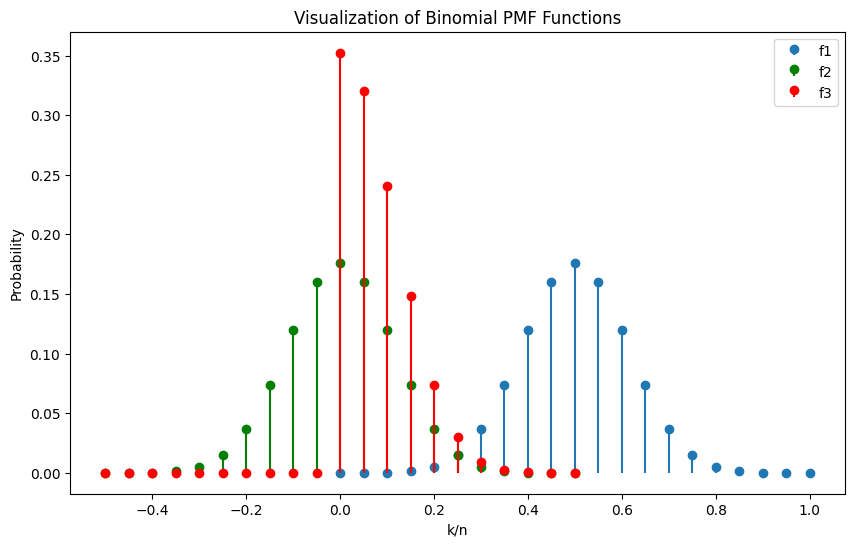
\includegraphics[width=0.7\textwidth]{figs/Visualization_of_Binomial_PMF_Functions.png}
    \caption{Visualization of Binomial PMF Functions}
    \label{fig:binomial_pmf}
\end{figure}

\begin{figure}[H]
    \centering
    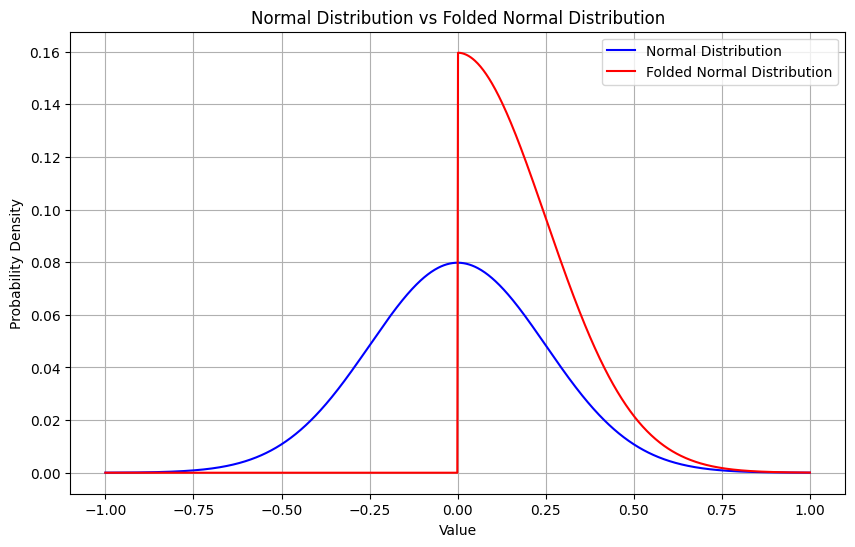
\includegraphics[width=0.7\textwidth]{figs/Normal Distribution_vs_Folded_Normal_Distribution.png}
    \caption{Normal Distribution vs Folded Normal Distribution}
    \label{fig:folded_normal_distribution}
\end{figure}


\subsubsection{The Set of Asymptotically Approachable Scores}

It is natural to ask what set of score functions $\hat{s}(\eta), 0 \leq \eta \leq 1$, satisfy (\ref{eq:4.8}) and (\ref{eq:4.9}) in the 
limit as $n \to \infty$. Clearly, the set of all continous differentiable such functions satisfies the constraints: 
\begin{equation}
    \hat{s}(\frac{1}{2}) = \frac{1}{2}
\end{equation}
\begin{equation}
    \left| \hat{s}(\eta) \right| < 1 , \quad 0 \leq \eta \leq 1
\end{equation}

We define the set of uniformly asymptotically approachable scores in the sense of Blackwell as follows:



\begin{equation}
    \begin{aligned}
        \hat{\mathcal{S}} = \left\{ \hat{s}(\eta), 0 \leq \eta \leq 1 : \exists p = (p_1, p_2, \ldots) \in \{0,1\}^\infty \text{ s.t. } \forall \Theta \in \{0,1\}^\infty \right. \\
        \left. \mathbb{P} \left\{ \lim_{n \to \infty} \left| \frac{1}{n} \sum_{i=1}^n s_i(\Theta_i) - \hat{s} \left( \frac{1}{n} \sum_{i=1}^n \Theta_i \right) \right| = 0 \right\} = 1 \right\}
    \end{aligned}
\end{equation}

(Recall that $s_i(\Theta_i) = \delta_i \Theta_i + (1 - \delta_i)(1 - \Theta_i)$ is a Random Variable govern by $p_i$.)

Blackwell reports that necessary and sufficient conditions for approachability and exclaudability are known only for convex functions. 

In particular, $\eta \alpha + (1 - \eta) (1 - \alpha)$, for $0 \leq \alpha \leq 1$, and $\max{\eta, 1 - \eta}$ are approachable.

\bigbreak

Cover offer the conjecture that $\hat{s}$ is approachable if and only if $\hat{s}\left(\frac{1}{2}\right) = \frac{1}{2}$ and
\[
\left| \hat{s}\left(\frac{k+1}{n}\right) - \hat{s}\left(\frac{k}{n}\right) \right| < \frac{1}{n},
\]
for all \( k = 0, 1, 2, \dots, n-1 \) and \( n = 1, 2, \dots \).







\newpage


% * * * * * * * * * * * * * * * * * * * * * * * * 
% * * * * * * * * * * * * * * * * * * * * * * * * 
% * * * * * * * * * * * * * * * * * * * * * * * * 
% * * * * * * * * * * * * * * * * * * * * * * * * 
% * * * * * * * * * * * * * * * * * * * * * * * * 
% * * * * * * * * * * * * * * * * * * * * * * * * 
% * * * * * * * * * * * * * * * * * * * * * * * * 
% * * * * * * * * * * * * * * * * * * * * * * * * 
% * * * * * * * * * * * * * * * * * * * * * * * * 
% * * * * * * * * * * * * * * * * * * * * * * * * 
% * * * * * * * * * * * * * * * * * * * * * * * * 
% * * * * * * * * * * * * * * * * * * * * * * * * 
% * * * * * * * * * * * * * * * * * * * * * * * * 
% * * * * * * * * * * * * * * * * * * * * * * * * 
% * * * * * * * * * * * * * * * * * * * * * * * * 
% * * * * * * * * * * * * * * * * * * * * * * * * 
% * * * * * * * * * * * * * * * * * * * * * * * * 
% * * * * * * * * * * * * * * * * * * * * * * * * 
% * * * * * * * * * * * * * * * * * * * * * * * * 
\section{Conclusions}




\end{document}